%Plantilla anteproyecto
%Última modificación: 21 de mayo de 2010
\documentclass[12pt,oneside,a4paper]{article}
\usepackage[spanish]{babel}
\usepackage[utf8]{inputenc}
\usepackage{graphicx}
\usepackage{float}
\usepackage{amsmath}
\usepackage{amssymb}
\usepackage{color}
\usepackage{colortbl}
\usepackage{subfigure}
\usepackage{url}
\usepackage[all]{xy}
\linespread{1}
\setlength{\parskip}{1\baselineskip}
\parindent 1cm
\sloppy


%Opciones que debes descomentar mientras estemos revisando el anteproyecto
%\usepackage{lineno}
%\linenumbers
\usepackage[pagebackref=true,breaklinks=true,letterpaper=true,colorlinks,bookmarks=true]{hyperref}


%lista de palabras que Latex no parte bien
\hyphenation{pa-la-bras lis-ta}

\begin{document}

\thispagestyle{empty}

\begin{center}


Departamento de Automática\\
Escuela Politécnica Superior\\
Universidad de Alcalá\\

\vspace{1cm}

%\includegraphics[width=4cm]{figuras/logo-uah.eps}

\textbf{ANTEPROYECTO}

\vspace{1cm}

\begin{large}\textbf{\textit{Presentación de una IA capaz de detectar información oculta en imágenes basada en esteganografía}}\end{large}

\vfill

Marzo - 2022

\end{center}

\begin{flushright}
\textit{Autor - \textbf{Sergio Sastre Arrojo}} \\
\textit{Director - \textbf{Miguel Ángel Sicilia Urbán}}
\end{flushright}

\newpage
\section{Introducción}

En la actualidad existen una gran variedad de ciberataques, y para cada ciberataque hay, a su vez, diversas vías por las que explotarlo. Estas vías se conocen como exploits y, dependiendo del objetivo, se podrán ejecutar o no. Para este trabajo queremos enfocarnos en un exploit en bastante típico que se suele usar para que el atacante pueda espiar a la víctima, recoger su información, infectar su red con un malware... nos referimos a los del tipo "Drive-By Download", más concretamente los "Drive-By Download Browser": este tipo de exploits se centran en ejecutar código desde el propio navegador con el que vulnerar el sistema objetivo.

Existen muchas formas de aplicar este exploit, sin embargo, vamos a basarnos en una de ellas bastante peligrosa (en gran parte por la sutileza que sugiere); nos referimos a la esteganografía, es decir, el arte de la ocultación de información a simple vista. Usando este método, el atacante puede introducir un código malicioso en una misma imagen sin que el usuario se dé cuenta y que éste se ejecute para comprometer el sistema. Para aplicar esta técnica usaremos stegosploits de Javascript. \cite{stegosploit}

Una solución que queremos presentar ante este tipo de infortunios es el uso de una IA lo suficientemente entrenada como para detectar estos códigos ocultos en imágenes, de forma que se pueda evitar, en la medida de lo posible, la infección del sistema.
%En los últimos años, con la aparición de los sistemas de adaptación inteligente de la velocidad (ISA), se han evitado muchas desgracias afortunadamente. No obstante, la tecnología actual viene con una serie de limitaciones que se podrían mejorar. Por ejemplo: la mayoría de estos sistemas utilizan GPS, lo cual es muy eficiente para su propósito, pero en determinadas ocasiones (núcleos urbanos, distinción de carriles en una autovía con una carretera de servicio) pueden desembocar en situaciones de gran peligro.

%¿Pero qué es un sistema ISA? ISA son las siglas de Intelligent Speed Adaptation, y como su propio nombre indica, es un sistema para adaptar la velocidad según diversos factores como: adaptación por proximidad con otros vehículos u objetos, o por GPS como hemos mencionado anteriormente.

%Es por ello que aquí presentamos una solución ante esos problemas: \[ISA^{2}\]

%Con este nuevo sistema queremos adaptar la velocidad del vehículo en base a la situación del tráfico en cada momento, la situación que el vehículo observa mediante una cámara frontal. Una primera aproximación a este problema ya ha sido implementada, y el principal objetivo de este TFG es mejorar ese sistema para hacerlo más preciso y práctico.


\section{Objetivos y campos de aplicación}

El objetivo principal de este proyecto es la aplicación de una solución eficaz en la detección de este tipo de ataques. En esencia, se pretende ayudar al usuario para evitar males mayores.

Por otro lado, podemos destacar los siguientes campos de aplicación para nuestro trabajo:
\begin{enumerate}
	\item Implementación de un sistema de detección de códigos en Javascript en imágenes.
	\item Desarrollo de nuevas ayudas en la protección del usuario en páginas web.
\end{enumerate}

En el siguiente apartado, explicaremos de forma breve el proceso que seguiremos para su realización.
%Como ya hemos dicho, el objetivo principal de este proyecto es optimizar la primera versión del sistema $ISA^{2}$.

%Para ello, realizaremos una repetición de los experimentos detallados en, para comprobar que las nuevas mejoras funciona correctamente y de forma más eficiente que el anterior.

%En cuanto a los campos de aplicación, cabrían destacar los siguientes:
%\begin{enumerate}
% \item Este proyecto será aplicable a cualquier campo relacionado con el automovilismo, para ayudar a mejorar la seguridad vial actual y para facilitar la lectura de la vía durante la conducción. En esencia, todo lo anterior se puede resumir en lo siguiente:
% \begin{enumerate}
% 	\item Implementación de soluciones de adaptación de velocidad inteligente.
% 	\item Implementación de sistema de detección de situaciones peligrosas en función de la velocidad.
% 	\item Desarrollo de nuevas ayudas a la conducción más inteligentes.
% \end{enumerate}
%\end{enumerate}



\section{Descripción del trabajo}

A continuación vamos a pasar a explicar las fases sobre las que se va a desarrollar el proyecto. Para ello nos ayudaremos de un diagrama de bloques:

\begin{figure}[h]
  \centering
  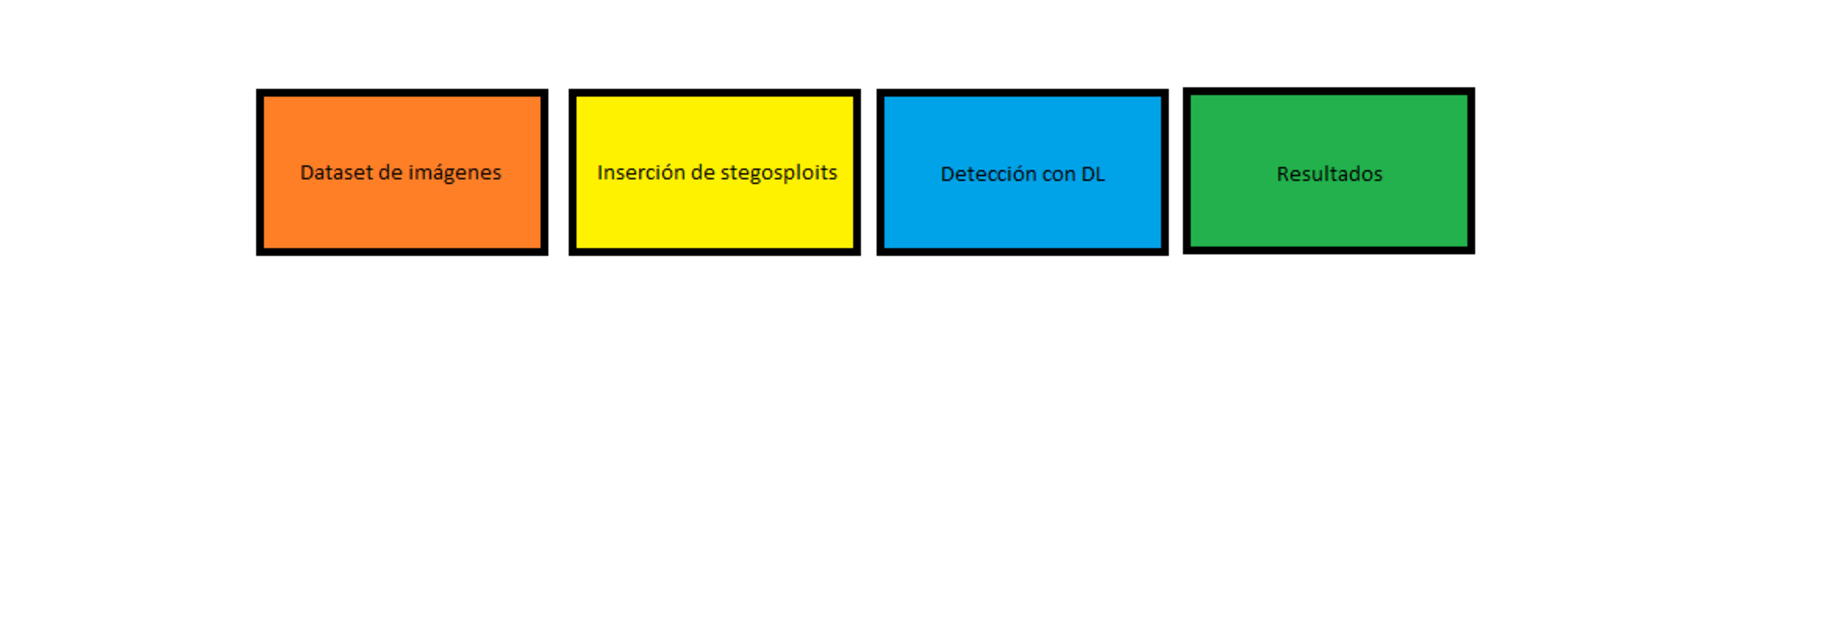
\includegraphics[width=16cm]{Descripcion_Trabajo.eps}
  \caption{Fases del proyecto}
  \label{fig:diagrama_bloques}
\end{figure}

Como se puede ver en la Figura, el trabajo se dividirá en 4 partes:

\begin{itemize}
	\item \textbf{Dataset de imágenes}
	
	En primer lugar, cogeremos una base de datos con diferentes imágenes para insertar los códigos con los stegosploits. Buscaremos entre las ya conocidas Cityscapes, Mapillary y Coco. \cite{cityscapes} \cite{mapillary} \cite{coco}
	\item \textbf{Inserción de stegosploits}
	
	A continuación, introduciremos los stegosploits de Javascript en las imágenes para poder trabajar con ellas en un modelo de Deep Learning.
	\item \textbf{Detección con DL}
	
	En este punto, vamos a trabajar con modelos de Deep Learning para la detección de estos códigos. En primer lugar los entrenaremos debidamente con un set de imágenes para, posteriormente, ejecutar una fase de evaluación y valorar los resultados obtenidos. Previo a todo esto, analizaremos en profundidad los modelos de Deep Learning que definen el estado del arte y, en consecuencia, trabajaremos con los que mejor se adapten a nuestros objetivos.
	\item \textbf{Resultados}
	
	Por último, concluiremos el trabajo con el análisis de los resultados obtenidos por los modelos y su valoración final para saber con cuanta exactitud se han detectado correctamente los códigos.
\end{itemize}

\section{Fases de desarrollo}

Teniendo en cuenta el apartado anterior, vamos a pasar a explicar de forma más detallada las diferentes fases del proyecto, además de su calendarización:

\begin{enumerate}
 \item Exploración de dataset de imágenes (1 semana)
 \item Integración de stegosploits de Javascript en el dataset (1 mes)
 \item Exploración de modelos de Deep Learning (1 semana)
 \item Entrenamiento de los modelos (1 mes)
 \item Realización de experimentos sobre el sistema para comprobar su funcionamiento (1 mes)
 \item Realización de memoria en LaTeX (Se realizará a lo largo de todo el cuatrimestre)
 \item Conclusiones (2 semanas)
 %Enumera, de forma esquemática los pasos en los que se traducen la descripción del trabajo que has escrito arriba. Tal y como venía en la plantilla que te pasé.
\end{enumerate}

\section{Medios disponibles}

Dispondremos de las siguientes herramientas:

\begin{enumerate}
	\item Estación de trabajo con GPU (NVIDIA Tesla) para la realización de experimentos.
	\item Acceso a Google Collab y otras nubes para entrenar modelos con GPUs.
	\item Acceso a diferentes librerías de Deep Learning:
	\begin{itemize}
	\item PyTorch
	\item Scikit-learn
	\item XGBoost
	\item LightGBM
	\end{itemize}
	%\item Acceso a la base de datos $ISA^2$ utilizada en la primera versión a través del siguiente enlace: \url{http://agamenon.tsc.uah.es/Personales/rlopez/data/isa2/index.html}.
\end{enumerate}

 
\bibliographystyle{plain}
\bibliography{Anteproyecto_TFM}


\end{document}
